\section{Preliminary Simulations}
	In order to test if RegCM5 is working on the laboratory's workstation,
		a preliminary simulation was conducted.
	The domain of the simulation is Luzon, centered on Manila, as shown in Figure \ref{fig:proposal-domain}.
	The domain has an area of $\num{130}$ by $\num{124}$ grid cells, with a $\qty{3}{km}$ resolution.
	Data for initial and boundary condition were dated from March to September 1990,
		and the simulation itself is from March to May 1990.
	The run used 24 cores and took 14 hours to complete.
		
	\begin{figure}
		\centering
		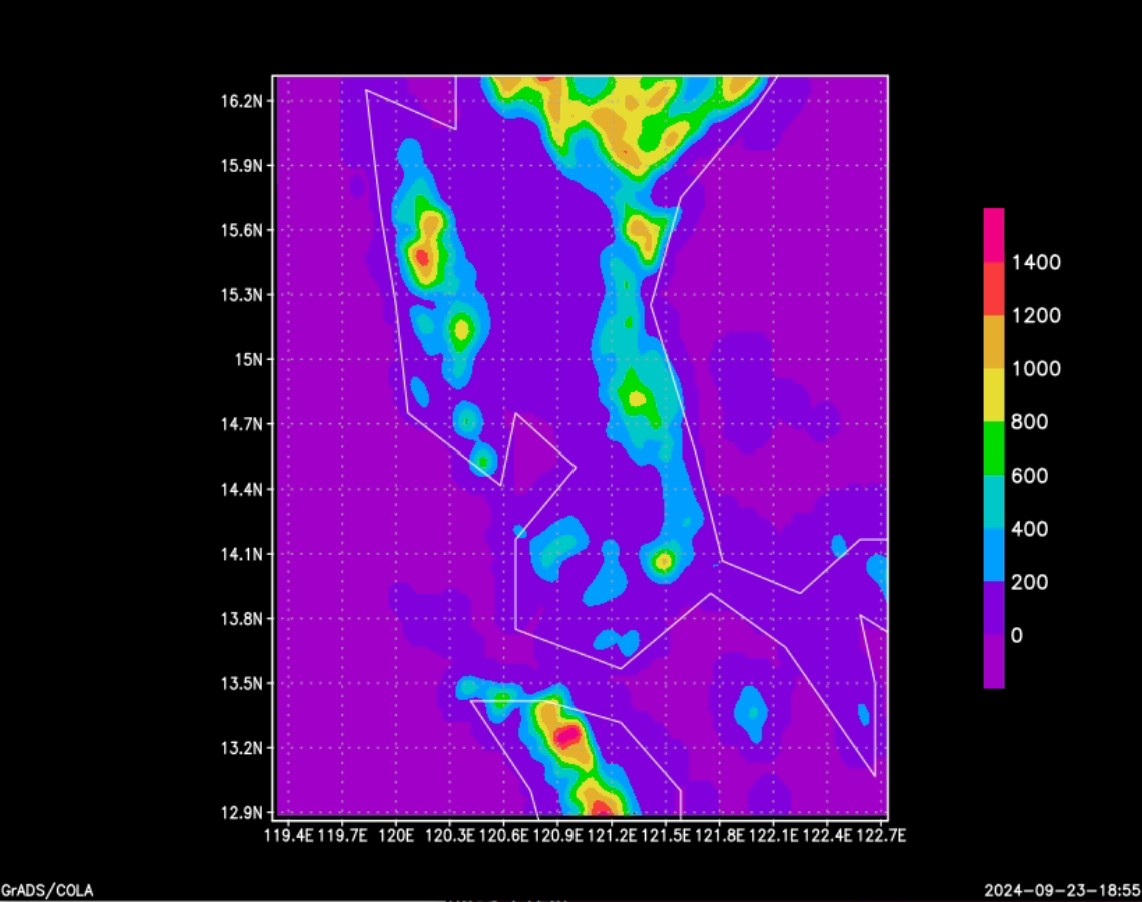
\includegraphics{proposal-domain}
		\caption{
			Surface model elevation of the domain used in the preliminary simulation.
			Domain is centered on Manila (\ang{14;35} N, \ang{121} E),
				with a grid of $\num{130}$ by $\num{124}$ cells
				and a resolution of $\qty{3}{km}$.
			Units of the elevation are in meters.
		}
		\label{fig:proposal-domain}
	\end{figure}
	
	Figure \ref{fig:proposal-manila-results} shows a comparison of the results of the simulation and the observed temperature in Manila for the month of March, 1990.
	Visually, the simulation somewhat matches the observed data, though there are large differences.
	Figures \ref{fig:proposal-naia-results} and \ref{fig:proposal-sciencegarden-results} show the same comparison as with Figure \ref{fig:proposal-manila-results}, 
		but for the Ninoy Aquino International Airport in Pasay City and the Science Garden in Quezon City, respectively.
	Visually, both cities exhibit higher simulated air temperature of around $+ \qty{2}{\degreeCelsius}$ compared to the observed data. 
	
	
	\begin{figure}
		\centering
		\begin{subfigure}{\textwidth}
			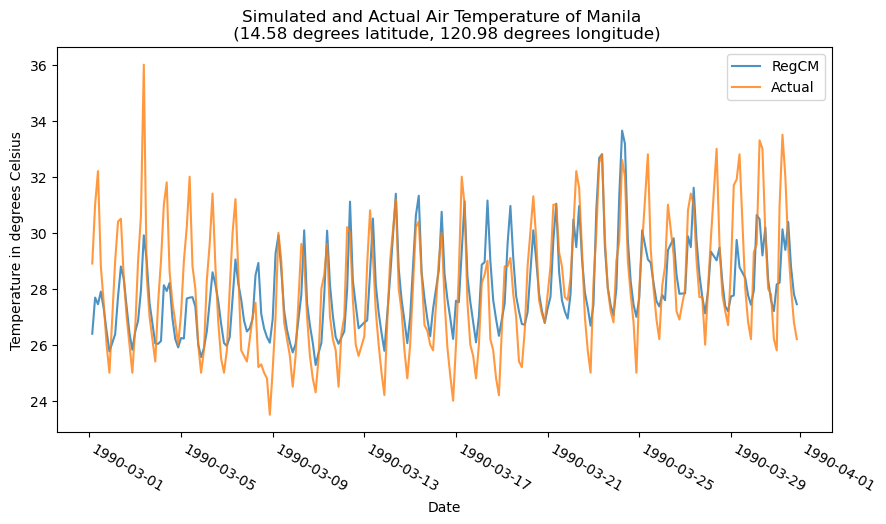
\includegraphics[width=\textwidth]{proposal-manila-both}
		\end{subfigure}
		\begin{subfigure}{\textwidth}
			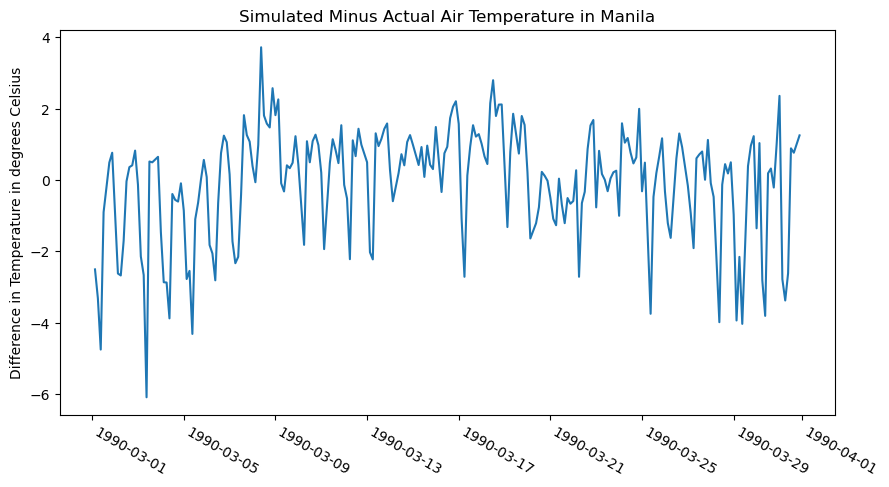
\includegraphics[width=\textwidth]{proposal-manila-difference}
		\end{subfigure}
		\caption{
			Graphs of the simulated and actual near-surface air temperature of Manila (\ang{14.58} N, \ang{120.98} E).
		}
		\label{fig:proposal-manila-results}
	\end{figure}
	
	\begin{figure}
		\centering
		\begin{subfigure}{\textwidth}
			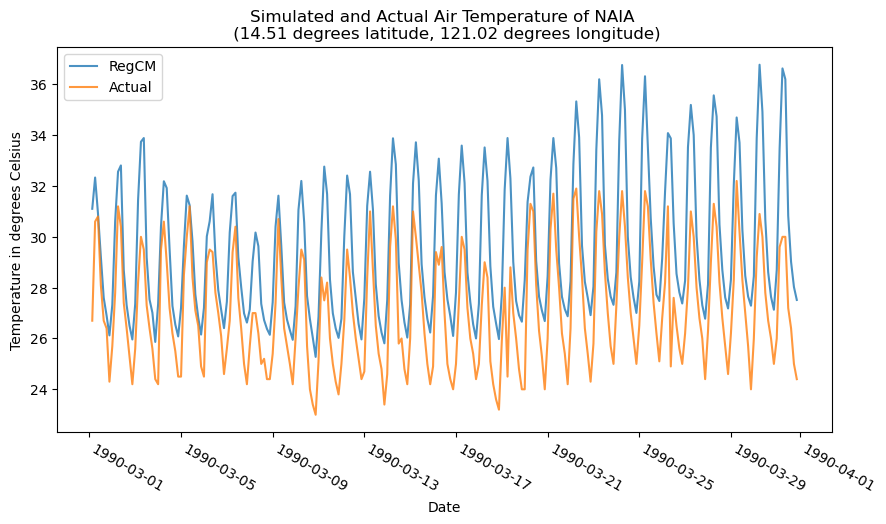
\includegraphics[width=\textwidth]{proposal-naia-both}
		\end{subfigure}
		\begin{subfigure}{\textwidth}
			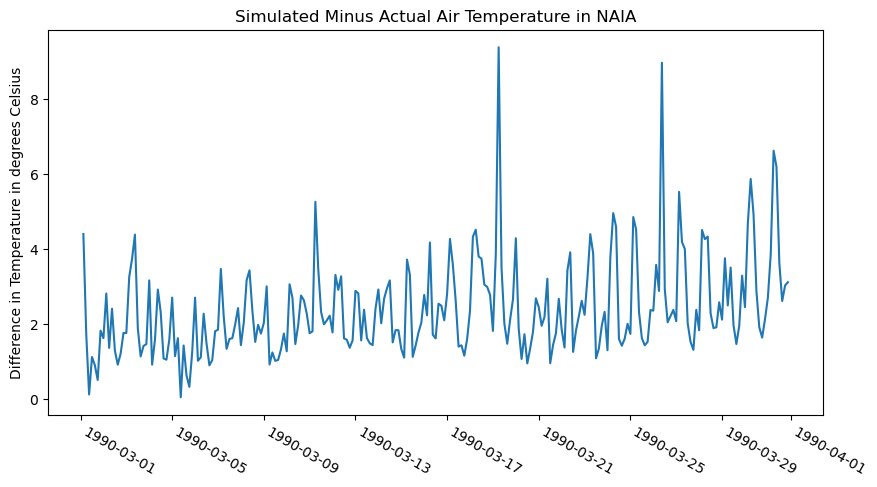
\includegraphics[width=\textwidth]{proposal-naia-difference}
		\end{subfigure}
		\caption{
			Graphs of the simulated and actual near-surface air temperature of the Ninoy Aquino International Airport, Pasay (\ang{14.51} N, \ang{120.02} E).
		}
		\label{fig:proposal-naia-results}
	\end{figure}

	\begin{figure}
		\centering
		\begin{subfigure}{\textwidth}
			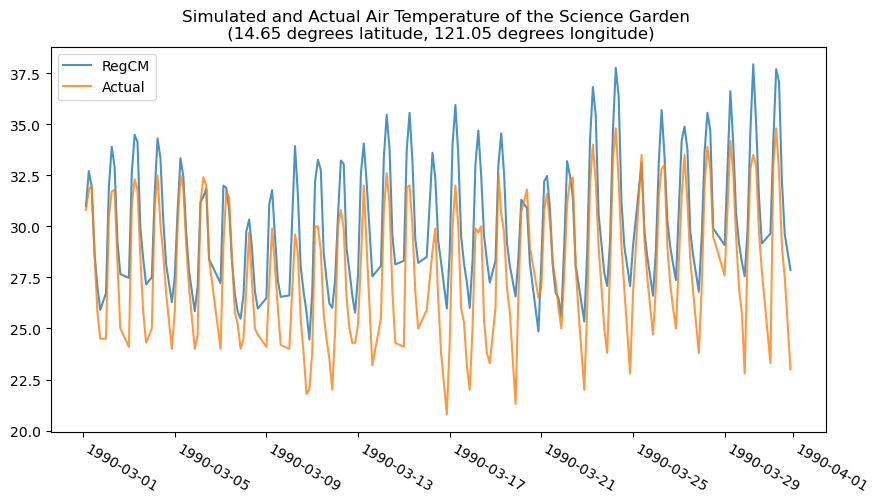
\includegraphics[width=\textwidth]{proposal-sciencegarden-both}
		\end{subfigure}
		\begin{subfigure}{\textwidth}
			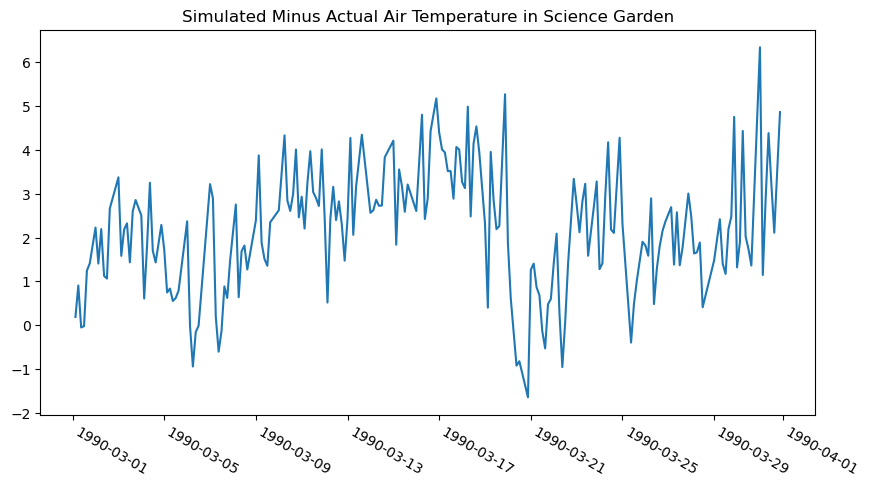
\includegraphics[width=\textwidth]{proposal-sciencegarden-difference}
		\end{subfigure}
		\caption{
			Graphs of the simulated and actual near-surface air temperature of the Science Garden, Quezon City (\ang{14.65} N, \ang{120.05} E).
		}
		\label{fig:proposal-sciencegarden-results}
	\end{figure}

\section{Expected Results}
	A map of the average air temperature of Metro Manila will be made, similar to Figure \ref{fig:rrl-almadronesreyes2022-mm}.
	A line graph of the air temperatures comparing the simulated and actual values will be made too, similar to Figures \ref{fig:proposal-manila-results} to \ref{fig:proposal-sciencegarden-results}.
	Evaluation of the simulation shall be performed and its results will be tabulated, together with a discussion of the findings.
	A sample table of the statistical performance of the simulation is given in Table \ref{tab:sample-statistical-performance}.
	The simulation of the present time period will take approximately a month to simulate.

	\begin{table}[]
		\caption{
			Sample table of the statistical performance of the simulation.
			Data taken from \textcite{Bilang2022}.
		}
		\label{tab:sample-statistical-performance}
		\centering
		\begin{tabular}{lrrrr}
			\hline \hline
			Location                    & MB (\unit{\degreeCelsius})    & MAE (\unit{\degreeCelsius}) & RMSE (\unit{\degreeCelsius}) & IOA \\
			\hline
			NAIA, Pasay City            & -0.91 & 1.15 & 1.40 & 0.90 \\
			Manila City                 & -0.09 & 0.68 & 0.98 & 0.94 \\
			Science Garden, Quezon City & 1.56  & 1.95 & 2.46 & 0.79 \\
			\hline
		\end{tabular}
	\end{table}

	The future.